\chapter{隐函数求导和相关变化率}
1.隐函数求导\\
例.\\
$x^2+y^2=4$\\[2ex]
推导过程:\\
设$u=y^2$, 则:\\
$\displaystyle\frac{\dif u}{\dif x}=\frac{\dif u}{\dif y}\frac{\dif y}{\dif x}=2y\frac{\dif y}{\dif x}$\\
原函数两边对$x$求导:\\[1ex]
$\displaystyle\frac{\dif }{\dif x}(x^2)+\frac{\dif }{\dif x}(y^2)=0\quad\Rightarrow\quad 2x+2y\frac{\dif y}{\dif x}=0\Rightarrow\frac{\dif y}{\dif x}=-\frac{x}{y}$\\[2ex]

2.隐函数求二阶导数\\
例.\\
$\displaystyle 2y+\sin(y)=\frac{x^2}{\pi}+1$\\[2ex]
推导过程:\\
设$u=\sin(y)$, 则:\\
$\displaystyle\frac{\dif u}{\dif x}=\frac{\dif u}{\dif y}\frac{\dif y}{\dif x}=\cos(y)\frac{\dif y}{\dif x}$\\
原函数两边对$x$求导:\\[1ex]
$\displaystyle 2\frac{\dif y}{\dif x}+\cos(y)\frac{\dif y}{\dif x}=\frac{2x}{\pi}\quad\Rightarrow\quad\frac{\dif y}{\dif x}=\frac{2x}{\pi(2+\cos(y))}$\\[1ex]
两边再次对$x$求导:\\[1ex]
$\displaystyle 2\frac{\dif ^2y}{\dif x^2}+\frac{\dif }{\dif x}\left(\cos(y)\frac{\dif y}{\dif x}\right)=\frac{2}{\pi}\quad\Rightarrow\quad 2\frac{\dif ^2y}{\dif x^2}-\sin(y)\left(\frac{\dif y}{\dif x}\right)^2+\cos(y)\frac{\dif ^2y}{\dif x^2}=\frac{2}{\pi}$\\
$\Rightarrow\displaystyle (2+\cos(y))\frac{\dif ^2y}{\dif x^2}-\sin(y)(\frac{\dif y}{\dif x})^2=\frac{2}{\pi}$\\[1ex]
将$\displaystyle\frac{\dif y}{\dif x}=\frac{2x}{\pi(2+\cos(y))}$带入结果:\\[1ex]
$\displaystyle (2+\cos(y))\frac{\dif ^2y}{\dif x^2}=\frac{2}{\pi}+\sin(y)\left(\frac{2x}{\pi(2+\cos(y))}\right)^2$\\
$\displaystyle\Rightarrow\quad\frac{\dif ^2y}{\dif x^2}=\frac{2}{\pi(2+\cos(y))}+\sin(y)\cdot\frac{4x^2}{\pi^2(2+\cos(y))^3}$\\[2ex]

3.相关变化率
{\par\centering
\framebox{如果$Q$是某个量, 那么$Q$的变化率是$\displaystyle\frac{\dif Q}{\dif t}$}\\[2ex]
\framebox{
\begin{minipage}[c]{10cm}
设$x=f(t)$和$y=g(t)$为两个变量的变化率, 由于$x$和$y$都是关于时间$t$的函数, 所以$x$与$y$必定存在某种关系, 这种关系称为\textbf{相对变化率}
\end{minipage}
}\par}

求解相关变化率的方法:\\
(1)识别出哪一个量需要求相关变化率;\\
(2)写出一个关联所有量的方程;\\
(3)对方程关于时间t做隐函数求导;\\
(4)将已知值带入方程中做替换.\\

例1.\\
用打气筒给一个完美球体的气球充气. 空气以常数速率$12\pi$立方英寸每秒进入气球.\\
(1)当气球的半径达到$2$英寸时, 气球的半径的变化率是多少?\\
(2)从外, 当气球的体积达到$36\pi$立方英寸时, 气球的半径的变化率又是多少?

解:\\
球体体积公式:\\[-2ex]
{\par\centering
\framebox{$\displaystyle V=\frac{4}{3}\pi r^3$}
\par}
方程对时间t进行隐式求导:
\begin{equation}
\displaystyle\frac{\dif V}{\dif t}=4\pi r^2\frac{\dif r}{\dif x}\label{eq:circle}
\end{equation}
(1)将$r=2$和$\frac{\dif V}{\dif t}=12\pi$代入公式\eqref{eq:circle}, 得:\\[1ex]
\phantom{(1)}$\displaystyle 4\pi\times 2^2\frac{\dif r}{\dif x}=12\pi\quad\Rightarrow\quad\frac{\dif r}{\dif x}=\frac{3}{4}$\\[1ex]
(2)根据球体体积公式, 得:\\[1ex]
\phantom{(2)}$\displaystyle\frac{4}{3}\pi r^3=36\pi\quad\Rightarrow\quad r=3$\\[1ex]
\phantom{(2)}将$r=3$和$\frac{\dif v}{\dif t}=12\pi$代入公式\eqref{eq:circle}, 得:\\[1ex]
\phantom{(2)}$\displaystyle 4\pi\times 3^2\frac{\dif r}{\dif x}=12\pi\quad\Rightarrow\quad\frac{\dif r}{\dif x}=\frac{1}{3}$\\[2ex]

例2.\\
假设有两辆汽车A和B. 汽车A在一条路上径直向北行驶远离你家, 而汽车B在另一条路上径直向西行驶接近你家. 汽车A以55英里/小时的速度行驶, 而汽车B以45英里/小时的速度行驶. 当A到达你家北面21英里, 而B到达你家东面28英里时, 两辆汽车间的距离的变化率是多少?

解:\\
如图.\\
\begin{tikzpicture}
\draw[color=white] (0,0) -- (5,0);
\draw[color=white] (0,0) -- (0,5);
\begin{scope}[xshift=3cm]
% 三角形
\draw[auto,swap] (0,0) node[below left=2mm]{H} -- node{b} (4,0) node[below=2mm]{B} -- node{c} (0,3) node[above left=2mm]{A} -- node{a} cycle;
% 小屋子
\begin{scope}[xshift=-3.5mm, yshift=1mm, scale=0.5]
\draw (0,0) -- (45:1);
\draw (45:2 |- 0,0) -- +(135:1);
\draw (45:0.3) -- (45:0.3 |- 0,-0.7);
\draw (45:2 |- 0,0) +(135:0.3) -- (45:1.7 |- 0,-0.7);
\draw (45:0.3 |- 0,-0.7) -- (45:1.7 |- 0,-0.7);
\draw (45:0.8 |- 0,-0.3) rectangle (45:1.2 |- 0,0);
\draw (45:2 |- 0,0) +(135:0.6) -- +(135:0.4) -- (45:1.6 |- 0,0.5) -- (45:1.4 |- 0,0.5) -- cycle;
\end{scope}
% 小货车
\begin{scope}[rotate=-90, xshift=-3cm, yshift=-1mm, scale=0.5]
\draw[rounded corners=3pt] (-1,0) rectangle (1,0.46);
\filldraw[fill=white] (-0.5,0.04) circle (0.19);
\filldraw[fill=white] (0.6,0.04) circle (0.19);
\draw[rounded corners=2pt] (-0.7,0.46) -- (-0.44,0.76) -- (-0.03,0.76) -- (-0.03,0.46);
\end{scope}
% 小汽车
\begin{scope}[xshift=4cm, yshift=-1.5mm, scale=0.5]
\draw[rounded corners=4pt] (-1,0) rectangle (1,0.4);
\filldraw[fill=white] (-0.6,0.05) circle (0.15);
\filldraw[fill=white] (0.6,0.05) circle (0.15);
\draw (-0.5,0.4) -- (-0.3,0.64) -- (0.3,0.64) -- (0.6,0.4);
\draw (0,0.4) -- (0,0.64);
\draw (0.25,0.64) -- (0.36,0.4);
\end{scope}
\end{scope}
\end{tikzpicture}\\
由图可知:\\
\[a^2+b^2=c^2\]
对时间t作隐函数求导:\\
\begin{equation}
2a\frac{\dif a}{\dif t}+2b\frac{\dif b}{\dif t}=2c\frac{\dif c}{\dif t}\label{eq:car}
\end{equation}
由于A在远离H, 所以距离随着时间增加:\\[1ex]
$\displaystyle\frac{\dif a}{\dif t}=55$\\[1ex]
而B在靠近H, 所以距离随着时间减少:\\[1ex]
$\displaystyle\frac{\dif b}{\dif t}=-45$\\[1ex]
将结果带入公式\eqref{eq:car}, 得:\\[1ex]
$\displaystyle\frac{\dif c}{\dif t}=-3$\\[2ex]

例3.\\
有一个奇怪的巨大的圆锥形水罐(锥尖在下方), 圆锥的高是圆锥半径的两倍. 如果水是以$8\pi$立方英尺/秒的速率注入水罐, 求:\\
(1)当水罐中水的体积为$18\pi$立方英尺时, 水位的变化率是多少?\\
(2)设想水罐底部有一个小洞, 致使水罐中每一立方英尺的水以一立方英尺每秒的速率流出. 当水罐中水的体积为$18\pi$立方英尺时, 水位的变化率是多少?

解:\\
如图.\\
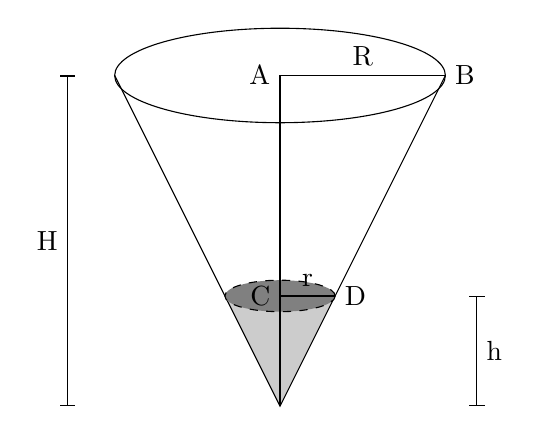
\begin{tikzpicture}
\draw (0,0) ellipse (21mm and 6mm);
\draw (21mm,0) -- (7mm,-28mm);
\draw (-21mm,0) -- (-7mm,-28mm);
\draw[fill=black!20] (-7mm,-28mm) -- (0,-42mm) -- (7mm,-28mm);
\draw[dashed, fill=black!50] (0,-28mm) ellipse (7mm and 2mm);
\draw (0,0) -- (0, -42mm);
\draw (0,0) node[left]{A} -- node[auto]{R} (21mm, 0) node[right]{B};
\draw (0,-28mm) node[left]{C} -- node[auto]{r} (7mm,-28mm) node[right]{D};
\draw[|-|] (-27mm,0) -- node[auto, swap]{H} (-27mm,-42mm);
\draw[|-|] (25mm,-28mm) -- node[auto]{h} (25mm,-42mm);
\end{tikzpicture}\\
圆锥体体积公式, 如下:
\[V=\frac{1}{3}\pi r^2h\]
(1)将$V=18\pi$, $r=\frac{h}{2}$代入体积公式, 得:\\[1ex]
\phantom{(1)}$\displaystyle\frac{1}{12}\pi h^3=18\pi\quad\Rightarrow\quad h=6$\\[1ex]
\phantom{(1)}将$r=\frac{h}{2}$代入体积公式, 并对结果两边关于时间t隐式求导, 得:\\[1ex]
\phantom{(1)}$\displaystyle\frac{\dif V}{\dif t}=\frac{\pi h^2}{4}\frac{\dif h}{\dif t}\quad\Rightarrow\quad 8\pi=9\pi\frac{\dif h}{\dif t}\quad\Rightarrow\quad\frac{\dif h}{\dif t}=\frac{8}{9}$\\[1ex]
(2)根据(1)得:\\
\phantom{(2)}$h=6$\\
\phantom{(2)}在当前秒, 水罐以$8\pi$立方英尺/秒注入水, 并以$18\pi$立方英尺/秒流出水, 所以:\\[1ex]
\phantom{(2)}$\displaystyle\frac{\dif V}{\dif t}=8\pi-18\pi=-10\pi$\\[1ex]
\phantom{(2)}将$r=\frac{h}{2}$代入体积公式, 并对结果两边关于时间t隐式求导, 得:\\[1ex]
\phantom{(2)}$\displaystyle\frac{\dif V}{\dif t}=\frac{\pi h^2}{4}\frac{\dif h}{\dif t}\quad\Rightarrow\quad -10\pi=9\pi\frac{\dif h}{\dif t}\quad\Rightarrow\quad\frac{\dif h}{\dif t}=-\frac{10}{9}$\\[2ex]

例4.\\
有一架飞机保持在$2000$英尺的高度远离你朝正东方向飞行. 飞机以$500$英尺每秒的常数速率飞行. 同时, 不久之前有一个跳伞员从直升飞机(它已经飞走了)上跳下来. 跳伞员在你东边$1000$英尺处上空垂直地以$10$英尺每秒的常数速率向下飘落, 跳伞员相对于你的方位角与飞机相对于你的方位角之差被标记为$\theta$. 求当飞机和跳伞员在同一高度, 但飞机在你东边$8000$英尺时, 角$\theta$的变化率是多少?\\
如图.\\
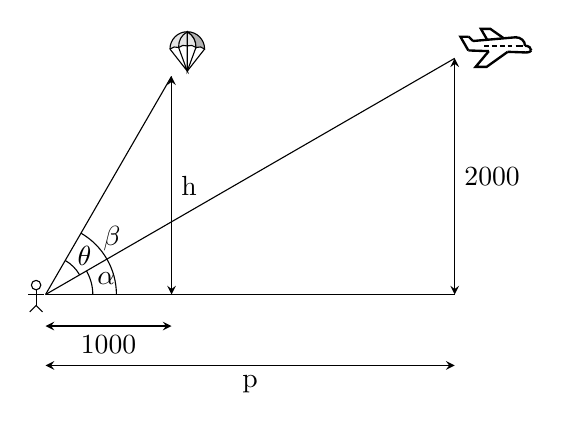
\begin{tikzpicture}
% 人
\begin{scope}[scale=0.2, shift=(180:6mm)]
\draw (-0.5,0) -- (0.5,0);
\draw (0,0.3) -- (0,-0.7);
\draw (0,0.6) circle[radius=0.3];
\draw (-0.4,-1.1) -- (0,-0.7) -- (0.4,-1.1);
\end{scope}
% 降落伞
\begin{scope}[shift=(60:3.6cm), scale=0.2]
\coordinate (a) at (-1.1cm,0);
\coordinate (b) at (-5.5mm,1mm);
\coordinate (c) at (0,2mm);
\coordinate (d) at (5.5mm,1mm);
\coordinate (e) at (1.1cm,0);
\coordinate (f) at (0,1.1cm);
\coordinate (g) at (0,-1.4cm);
\draw[fill=black!10] (a) to[bend left] (b) to[bend left] (c) to[bend left] (d) to[bend right] (f) arc[start angle=90, end angle=180, radius=1.1cm];
\draw[fill=black!30] (f) to[bend left] (d) to[bend left] (e) arc[start angle=0, delta angle=90, radius=1.1cm];
\draw (c) to (f) to[bend right] (b);
\draw (a) to (g) to (b);
\draw (c) to (g) to (d);
\draw (g) to (e);
\end{scope}
% 飞机
\begin{scope}[line width=0.3mm, shift=(30:6.2cm), scale=0.2]
\draw (0,0) -- (-2:1.3);
\draw (-2:2.5) -- (-2:3.6);
\draw (0.3,0.6) -- +(5:2.8);
\draw (0.3,0.6) -- +(135:0.4);
\draw (0,0) -- (120:1) -- +(0.52,0);
\draw (3.6,0.3) arc (0:90:0.6 and 0.54);
\draw (4.0,0) arc (0:90:0.4 and 0.3);
\draw (4.0,0) arc (0:-90:0.4 and 0.13);
\draw (1,0.3) -- ++(0.3,0) ++(0.2,0) -- ++(0.3,0) ++(0.2,0) -- ++(0.3,0) ++(0.2,0) -- +(0.3,0);
\draw (3,0.3) -- +(0.5,0);
\draw (-2:1.3) -- ++(230:1.3) -- +(0.7,0) -- (-2:2.5);
\draw (0.3,0.6) ++(5:0.9) -- ++(120:0.8) -- ++(0.6,0) -- +(-35:1);
\end{scope}
% 人与降落伞组成的三角形
\draw (0,0) -- (60:3.2cm);
\draw[stealth-stealth] (60:3.2cm) -- (60:3.2cm |- 0,0) node[auto, pos=0.5]{h};
% 人与飞机组成的三角形
\draw (0,0) -- (30:6cm);
\draw (0,0) -- (30:6cm |- 0,0);
\draw[stealth-stealth] (30:6cm) -- (30:6cm |- 0,0) node[auto, pos=0.5]{2000};
% 飞机-人连线与降落伞-人连线组成的夹角
\draw (30:5mm) arc [start angle=30, end angle=60, radius=5mm];
\node at (45:7mm) {$\theta$};
% 飞机与水平线组成的夹角
\draw (0:6mm) arc [start angle=0, end angle=30, radius=6mm];
\node at (15:8mm) {$\alpha$};
% 降落伞与水平线组成的夹角
\draw (0:9mm) arc [start angle=0, end angle=60, radius=9mm];
\node at (40:11mm) {$\beta$};
% 辅助线
\draw[<->, >=stealth] (60:3.2cm |- 0,0) +(0,-4mm) -- (0,-4mm) node[auto, pos=0.5]{1000};
\draw[<->, >=stealth] (30:6cm |- 0,0) +(0,-9mm) -- (0,-9mm) node[auto, pos=0.5]{p};
\end{tikzpicture}\\
由图可知:\\
\begin{gather}
\tan(\alpha)=\frac{2000}{p}\label{change_ratio:1}\\
\tan(\beta)=\frac{h}{1000}\label{change_ratio:2}\\
\theta=\beta-\alpha\label{change_ratio:3}
\end{gather}
公式\eqref{change_ratio:1}两边对时间t进行隐式求导:\\[1ex]
$\displaystyle\sec^2(\alpha)\frac{\dif \alpha}{\dif t}=-\frac{2000}{p^2}\frac{\dif p}{\dif t}\quad\Rightarrow\quad(\tan^2(\alpha)+1)\frac{\dif \alpha}{\dif t}=-\frac{2000}{8000^2}\frac{\dif p}{\dif t}\quad\Rightarrow$\\[1ex]
$\displaystyle\frac{\dif \alpha}{\dif t}=-\frac{1}{32000}\times 500\times\frac{16}{17}\quad\Rightarrow\quad\frac{\dif \alpha}{\dif t}=-\frac{1}{68}$\\[1ex]
公式\eqref{change_ratio:2}两边对时间t进行隐式求导:\\[1ex]
$\displaystyle\sec^2(\beta)\frac{\dif \beta}{\dif t}=\frac{1}{1000}\frac{\dif h}{\dif t}\quad\Rightarrow\quad(\tan^2(\beta)+1)\frac{\dif \beta}{\dif t}=-\frac{1}{100}\quad\Rightarrow$\\[1ex]
$\displaystyle\frac{\dif \beta}{\dif t}=-\frac{1}{100}\times\frac{1}{5}\quad\Rightarrow\quad\frac{\dif \beta}{\dif t}=-\frac{1}{500}$\\[1ex]
公式\eqref{change_ratio:3}两边对时间t进行隐式求导:\\[1ex]
$\displaystyle\frac{\dif \theta}{\dif t}=\frac{\dif \beta}{\dif t}-\frac{\dif \alpha}{\dif t}=-\frac{1}{500}+\frac{1}{68}=\frac{-17+125}{8500}=\frac{27}{2125}$\\[1ex]
